% Activate the following line by filling in the right side. If for example the name of the root file is Main.tex, write
% "...root = Main.tex" if the chapter file is in the same directory, and "...root = ../Main.tex" if the chapter is in a subdirectory.

%!TEX root =  ../../Tesis.tex
\chapter{An�lisis de selecci�n positiva en prote�nas codificadas por nDNA}\label{anexo:MetnDNA}

En el cap�tulo \ref{cap:Met} se llevaron a cabo an�lisis sobre las prote�nas codificadas por mtDNA para observar el efecto de la composici�n nucleot�dica sobre el contenido de ciste�na, metionina y treonina. De igual forma, en este ap�ndice se muestran los resultados de los mismos an�lisis aplicados sobre 61 prote�nas codificadas por nDNA pertenecientes a una docena de especies de mam�feros (figura \ref{Fig:nDNA}). Se observa que, mientras ${\Delta}$Met $>$ 0 en todas las especies analizadas, los valores de ${\Delta}$Cys y ${\Delta}$Thr fueron negativos en todos los casos. Estos resultados podr�an sugerir la presencia de selecci�n positiva sobre la abundancia de metionina tambi�n en el caso de las prote�nas codificadas por nDNA. No obstante, dado el escaso n�mero de especies computadas, no se pueden arrojar conclusiones s�lidas.

% Figura nDNA
\begin{figure}
\begin{center}
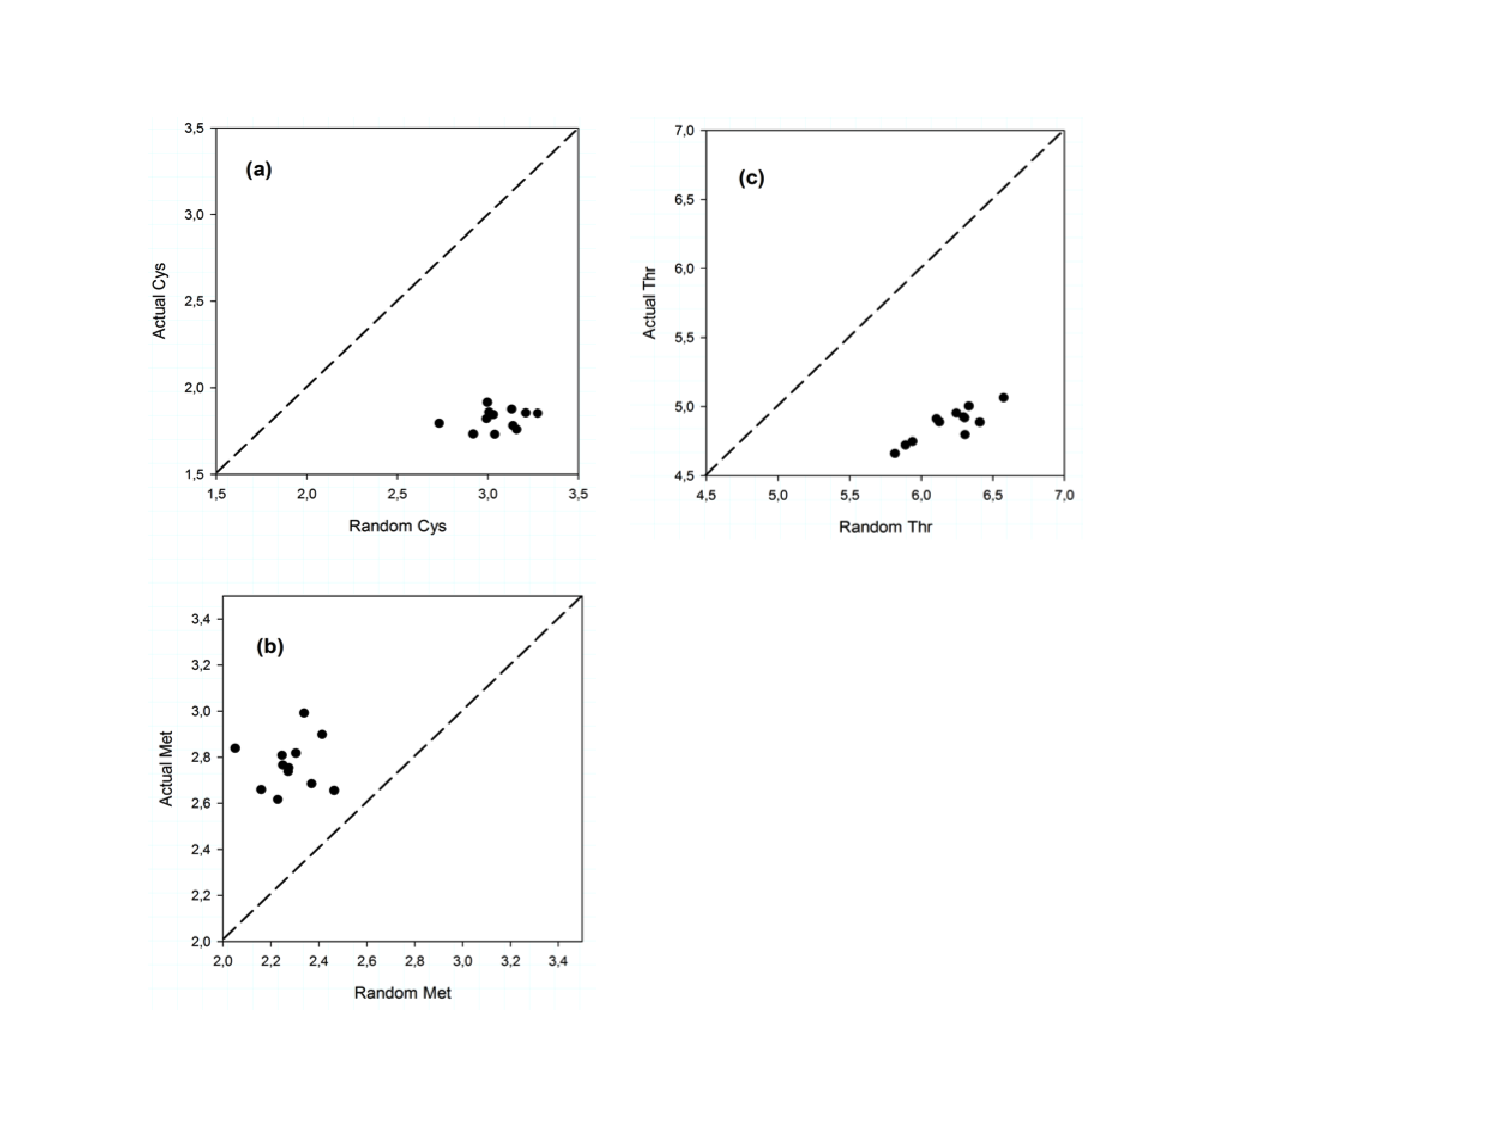
\includegraphics[width=1\textwidth]{Apendices/nDNA/Figuras/nDNA.pdf}
\end{center}
\caption{\small{Comparaci�n entre la abundancia aminoac�dica medida en las prote�nas originales codificadas por nDNA y lo esperado por la �nica influencia de la composici�n nucle�tidica. Para llevar a cabo este an�lisis se usaron 61 genes nucleares que codifican para prote�nas pertenecientes a los complejos I, III y IV de la cadena transportadora de electrones de 12 mam�feros distintos (\textit{Ailuropoda melanoleuca}, \textit{Bos taurus}, \textit{Canis familiares}, \textit{Equus caballus}, \textit{Homo sapiens}, \textit{Macaca mulatta}, \textit{Monodelphis domestica}, \textit{Mus musculus}, \textit{Pongo abelii}, \textit{Pan troglodites}, \textit{Rattus norvegicus}, \textit{Sus scrofa}). Para cada especie, se comput� el n�mero de ciste�nas (a), metioninas (b) y treoninas (c) presentes en las prote�nas originales y se represent� gr�ficamente frente al n�mero de veces que el correspondiente amino�cido aparece codificado en la secuencia aleatoria, la cual presenta la misma composici�n nucleot�dica que la original.}}
\label{Fig:nDNA}
\end{figure}
% Fin de nDNA